\documentclass{article}
\renewcommand{\baselinestretch}{1.25}

\usepackage{xeCJK}  % support character

% monokai code
\usepackage{color}
\usepackage{minted}
\usemintedstyle{manni}
\setminted{
    linenos,
    fontsize=\footnotesize,
    resetmargins
}

% insert images
\usepackage{graphicx}
\graphicspath{{images/}{../images/}}
\usepackage{amsmath}
\usepackage{caption}
\numberwithin{figure}{section}
\numberwithin{table}{section}
\numberwithin{listing}{section}
\numberwithin{equation}{section}

\usepackage{subcaption}

% hyperlink
\usepackage{hyperref}
\usepackage{xcolor}
\hypersetup{
    colorlinks,
    linkcolor={red!50!black},
    citecolor={blue!50!black},
    urlcolor={blue!80!black}
}

% auto newline in table
\newcommand{\tabincell}[2]{\begin{tabular}{@{}#1@{}}#2\end{tabular}}
\usepackage{multirow}

\usepackage{mathtools}
\usepackage{amsfonts}

\author{郭一隆(2013011189)}
\title{连连看实验报告}

\begin{document}
    \maketitle

    \tableofcontents
    \newpage

    \listoffigures
    \listoftables
    \renewcommand\listoflistingscaption{List of Source Codes}
    \listoflistings
    \newpage

    \section{原创性} % (fold)
    \label{sec:原创性}
        
        \textbf{本次连连看大作业由本人独立思考完成,如有雷同,纯属巧合。}

    % section 原创性 (end)

    \section{制作自己的连连看} % (fold)
    \label{sec:制作自己的连连看}
    
        \begin{enumerate}
            \item 在\texttt{MATLAB}环境下,设置当前路径为\texttt{linkgame},运行\texttt{linkgame}(打开\href{../linkgame/linkgame.fig}{\texttt{linkgame.fig}}或右键\href{../linkgame/linkgame.p}{\texttt{linkgame.p}}点“运行”),熟悉游戏。

                \begin{figure}[H]
                    \centering
                    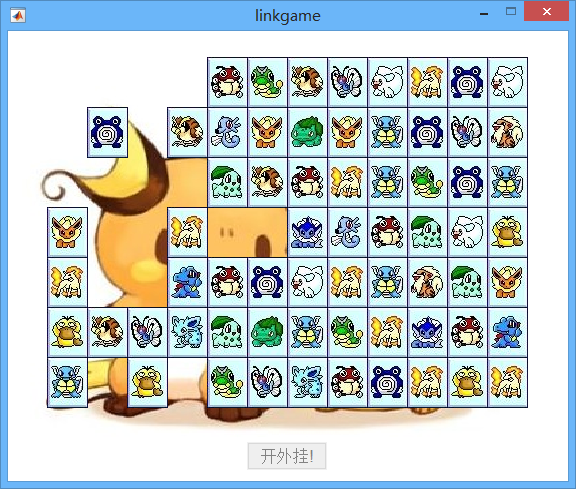
\includegraphics[width=0.7\textwidth]{run_linkgame}
                    \caption{运行连连看}
                \end{figure}

            \item 注意\texttt{linkgame}目录下有个\texttt{detect.p},它的功能时检测块是否可以消除。现将其删掉,然后把\texttt{linkgame\textbackslash reference}目录下的\href{../linkgame/reference/detect.m}{\texttt{detect.m}}复制到\texttt{linkgame}目录下。\href{../linkgame/detect.m}{\texttt{detect.m}}文件中是\texttt{detect}函数,函数以图像块的索引矩阵与要判断的两个块的下标为输入,如果两个块能消掉则输出\texttt{1},否则输出\texttt{0}。根据文件中的注释提示,实现判断块是否可以消除的功能。写完后再次运行\texttt{linkgame},检验游戏是否仍然可以正确运行。

                算法实现分为以下几个步骤:

                \begin{enumerate}
                    \item \textbf{画十字\texttt{adjcross}}:在给定点周围空白处画十字,遇到块则停止。

                        \begin{listing}[H]
                            \inputminted[firstline=29, lastline=48]{matlab}{../linkgame/canlink.m}
                            \caption{\texttt{canlink.m(adjcross)}}
                        \end{listing}

                    \item \textbf{判断是否可直连\texttt{canlink0}}:先判断横纵坐标是否在同一直线,再确认路径上是否有障碍。

                        \begin{listing}[H]
                            \inputminted[firstline=51, lastline=62]{matlab}{../linkgame/canlink.m}
                            \caption{\texttt{canlink.m(canlink0)}}
                        \end{listing}

                    \item \textbf{判断是否可用不超过一个直角的连线连接\texttt{canlink1}}:选取两目标点之一作为起点,画十字;对十字上的点进行遍历,检查是否存在可与另一目标点直连的点。

                        \begin{listing}[H]
                            \inputminted[firstline=65, lastline=86]{matlab}{../linkgame/canlink.m}
                            \caption{\texttt{canlink.m(canlink1)}}
                        \end{listing}

                    \item \textbf{判断可连性\texttt{canlink}}:选取两目标点之一作为起点,画十字;对十字上的点进行遍历,检查是否存在可与另一目标用不超过一个直角的连线连接的点。

                        \inputminted[firstline=1, lastline=26]{matlab}{../linkgame/canlink.m}
                        \begingroup
                            \captionof{listing}{\texttt{canlink.m(main)}}
                        \endgroup
                \end{enumerate}

                再次运行\texttt{linkgame},\href{../linkgame/detect.m}{\texttt{detect.m}}功能正常。

                \begin{minted}{matlab}
function bool = detect(mtx, x1, y1, x2, y2)
    
    [m,n] = size(mtx);
    
    % add surrounding zeros
    mtx = [0,zeros(1,n),0;
        zeros(m,1),mtx,zeros(m,1);
        0,zeros(1,n),0];
    
    origin = mtx(x1+1,y1+1);
    target = mtx(x2+1,y2+1);
    
    if origin == target && canlink(mtx,x1+1,y1+1,x2+1,y2+1)
        bool = 1;
    else
        bool = 0;
    end
       
end
                \end{minted}
                \begingroup
                    \captionof{listing}{\texttt{detect.m(main)}}
                \endgroup

                \begin{figure}[H]
                    \centering
                    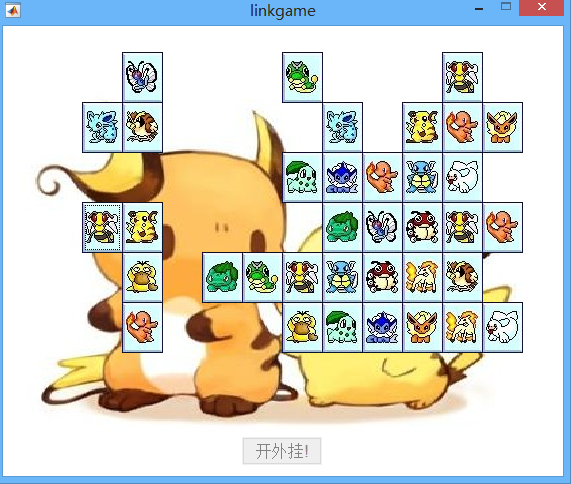
\includegraphics[width=0.7\textwidth]{mydetect_linkgame}
                    \caption{重写\texttt{detect.m}后运行\texttt{linkgame}}
                \end{figure}

            \item “外挂”模式逐一自动消除所有的块的功能是由\texttt{link}目录的\texttt{omg.p}实现的。删掉\texttt{omg.p}重新实现\href{../linkgame/omg.m}{\texttt{omg.m}}。

                根据游戏经验,算法通过以下几个步骤实现:

                \begin{enumerate}
                    \item \textbf{消去相邻的相同块\texttt{matchadj}}:利用自带函数\texttt{diff}实现,注意及时更新原矩阵以及保证多个相同块连续相邻时仍正确工作。

                        \inputminted[firstline=42,lastline=76]{matlab}{../linkgame/omg.m}
                        \begingroup
                            \captionof{listing}{\texttt{omg.m(matchadj)}}
                        \endgroup

                        \begin{figure}[H]
                            \centering
                            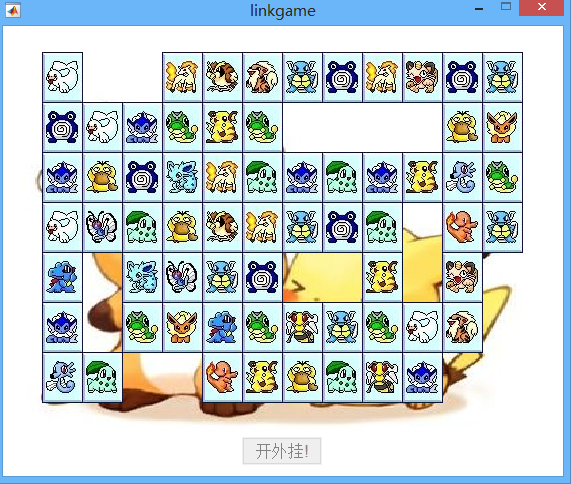
\includegraphics[width=0.7\textwidth]{match_adjacent}
                            \caption{测试\texttt{matchadj()}功能}
                        \end{figure}

                        \texttt{matchadj}函数工作正常。

                    \item \textbf{消去同一条边界上的相同块\texttt{matchborder}}:先定义\textbf{上边界},如图\ref{fig:upper_border}中的\textcolor{blue}{蓝色区域}。

                        \begin{figure}[H]
                            \centering
                            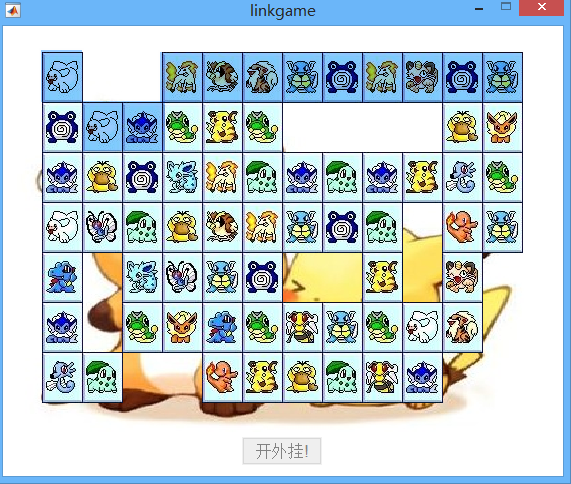
\includegraphics[width=0.7\textwidth]{upper_border}
                            \caption{定义上边界}
                            \label{fig:upper_border}
                        \end{figure}

                        显然,\textbf{上边界即每一列第一个非零元素};类似地可以定义其他边界。

                        容易证明,\textbf{在同一边界上的相同块必然可消去}。

                        与\texttt{matchadj}不同,由于消去过程会使边界发生变化,故必须不断循环直至边界保持不变。则实现\texttt{matchborder}函数如下:

                        \inputminted[firstline=79,lastline=135]{matlab}{../linkgame/omg.m}
                        \begingroup
                            \captionof{listing}{\texttt{omg.m(matchborder)}}
                        \endgroup

                        \begin{figure}[H]
                            \centering
                            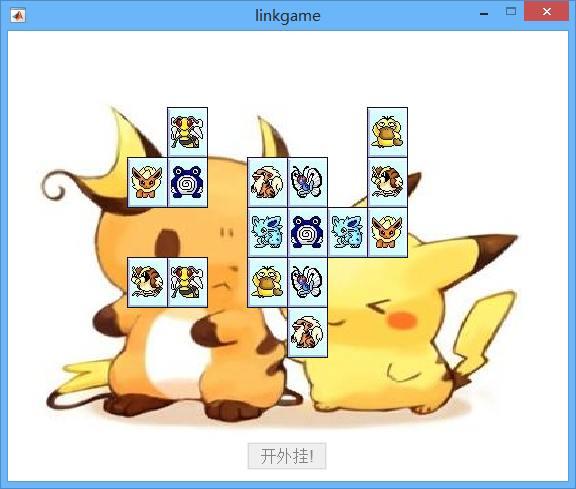
\includegraphics[width=0.7\textwidth]{match_border}
                            \caption{依次调用\texttt{matchadj}和\texttt{matchborder}后}
                            \label{fig:match_border}
                        \end{figure}

                        经过多次测试,发现\texttt{matchadj}与\texttt{matchborder}相结合的算法已经能消去游戏区域的\textbf{绝大多数块},甚至有时可\textbf{全部消去}。

                        \texttt{matchadj}的核心是\texttt{MATLAB}自带的\texttt{diff}函数,效率较高;

                        而\texttt{matchborder}通过\texttt{cumsum}以及\texttt{sum}函数巧妙获得各边界索引,再利用\texttt{unique}以及\texttt{find}等方法在边界内寻找相同的块,可以说十分高效。

                        既然高效的前两步已可以消去大多数块,那么对于剩余的块,不妨采取较暴力的算法解决。

                    \item \textbf{对于剩余的块按种类遍历尝试连接\texttt{matchrest}}:这里假设生成的连连看游戏是可以以任意消除顺序完全消除的(实践观测结果如此)。

                        \inputminted[firstline=138,lastline=164]{matlab}{../linkgame/omg.m}
                        \begingroup
                            \captionof{listing}{\texttt{omg.m(matchrest)}}
                        \endgroup

                        经过多次测试,均能顺利完成功能。

                        \begin{listing}[H]
                            \begin{minted}{matlab}
function steps = omg(mtx)
    
    [m,n] = size(mtx);
    
    % add surrounding zeros
    mtx = [0,zeros(1,n),0;
        zeros(m,1),mtx,zeros(m,1);
        0,zeros(1,n),0];
    
    [steps1,mtx] = matchadj(mtx);
    [steps2,mtx] = matchborder(mtx);
    [steps3,mtx] = matchrest(mtx);
    steps = [steps1,steps2,steps3];
    
    % make steps meet interface
    steps = [length(steps)/4,steps-1];

end
                            \end{minted}
                            \caption{\texttt{omg.m(main)}}
                        \end{listing}

                \end{enumerate}

        \end{enumerate}

    % section 制作自己的连连看 (end)

    \newpage
    \section{攻克别人的连连看} % (fold)
    \label{sec:攻克别人的连连看}

        \begin{enumerate}
            \item 在\texttt{MALTAB}环境下,将路径设置到\texttt{process}文件夹下。对游戏区域的屏幕截图(灰度图像)\href{../process/graygroundtruth.jpg}{\texttt{graygroundtruth}}进行分割,提取所有图像分块。

                先进行预处理:

                \begin{minted}{matlab}
%% load image and preprocess
original = imread('graygroundtruth.jpg');
image = double(original);
image = image - 128;
                \end{minted}

                绘制水平竖直扫描线灰度均值如图\ref{fig:gray_mean}。

                \begin{figure}[H]
                    \centering
                    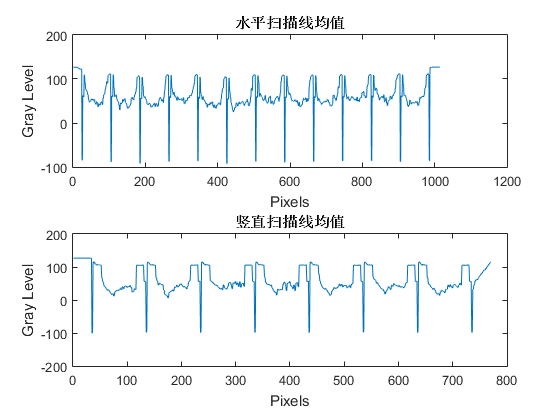
\includegraphics[width=0.7\textwidth]{gray_mean}
                    \caption{扫描线灰度均值}
                    \label{fig:gray_mean}
                \end{figure}

                周期如此明显,可以通过一些简单的运算直接获得块大小\texttt{(Wb,Hb)}、游戏区域位置信息\texttt{(Xs,Ys)}以及块数量\texttt{(Nc,Nr)}(而不需要进行傅里叶变换)。

                \begin{minted}{matlab}
%% get block size and position of game region
hor = mean(image,1);
ver = mean(image,2);

npeak = min(hor); % negative peak
I = find(hor<0.9*npeak);
I = sort(I);
Xs = I(1);
I = diff(I); % width between peaks
I = I(I>30); % filter too small blocks
Wb = mean(I)+1;
Nc = length(I); % number of block columns

npeak = min(ver); % negative peak
I = find(ver<0.9*npeak);
I = sort(I);
Ys = I(1);
I = diff(I); % width between peaks
I = I(I>30); % filter too small blocks
Hb = mean(I)+1;
Nr = length(I); % number of block rows
                \end{minted}
                \begingroup
                    \captionof{listing}{\texttt{divide.m}获取块大小以及位置信息}
                \endgroup

                然后按得到的尺寸\texttt{(Xs=25, Ys=35, Wb=80, Hb=100, Nc=12, Nr=7)}获取各图像块,效果良好:

                \begin{listing}[H]
                    \inputminted[firstline=20,lastline=31]{matlab}{../process/divide.m}
                    \caption{\texttt{divide.m}获取所有块}
                    \label{code:all_blocks}
                \end{listing}

                \begin{figure}[H]
                    \centering
                    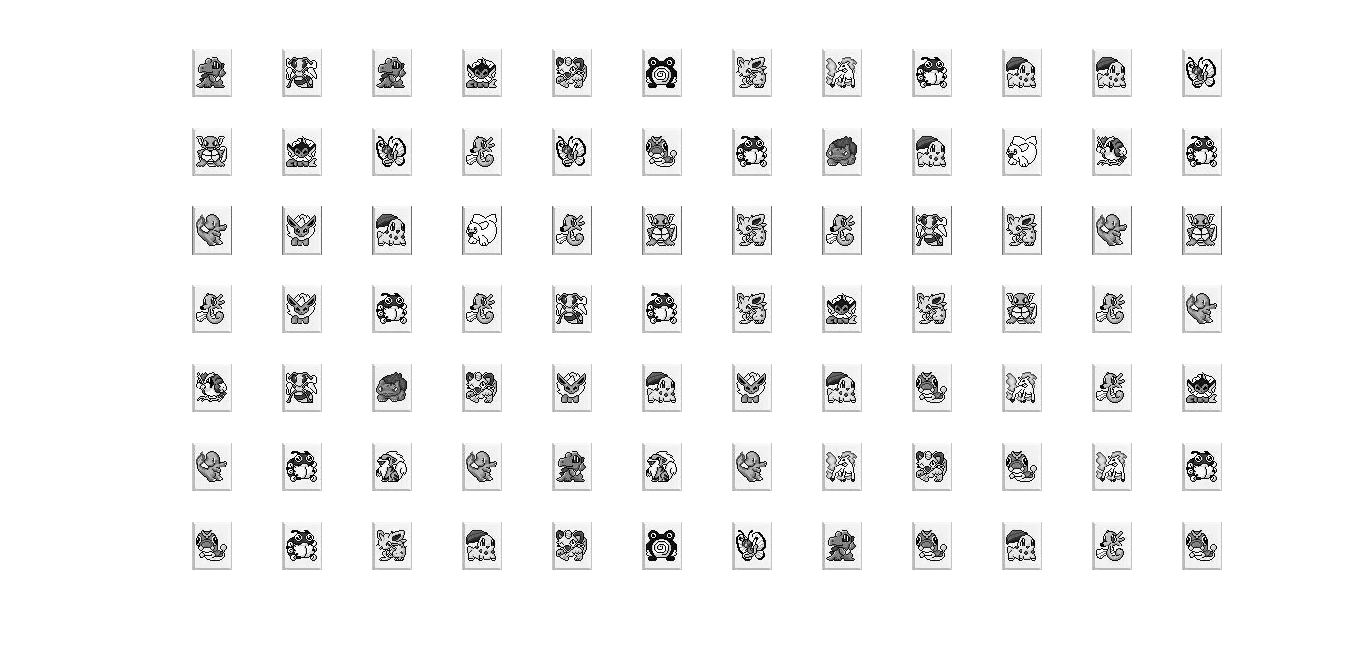
\includegraphics[width=\textwidth]{all_blocks}
                    \caption{图像分割效果}
                \end{figure}

            \item 对摄像头采集的图像(灰度图像)\href{../process/graycapture.jpg}{\texttt{graycapture}},参考第1题要求进行处理。

                摄像头采集的图像噪音明显增多,而且图像有小幅度的旋转。上一题使用的方法在这里完全不能获得正确结果。

                另外,画面对比度较弱,使得横纵方向的周期性也不明显了。

                考虑将其转化为二值图像(黑白图像)以增强周期性。

                预处理:

                \begin{minted}{matlab}
%% load image and preprocess
original = imread('graycapture.jpg');
image = im2bw(original,0.8);   % convert to bw image
image = double(image);
                \end{minted}

                \begin{figure}[H]
                    \centering
                    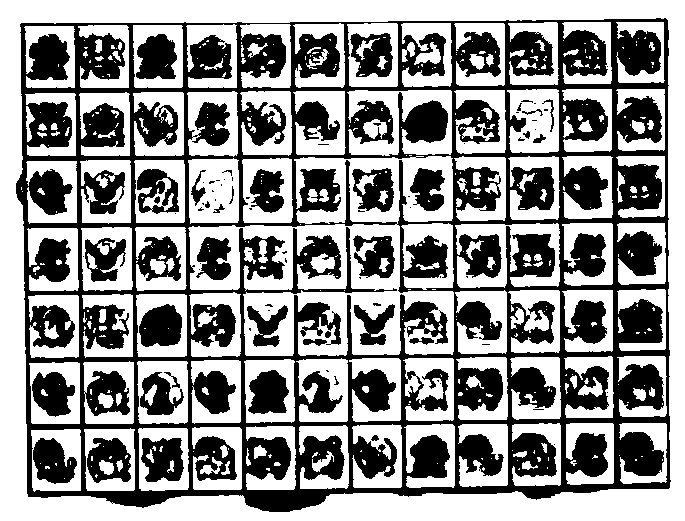
\includegraphics[width=0.7\textwidth]{graycapture_bw}
                    \caption{\texttt{graycapture}预处理成黑白图像}
                    \label{fig:graycapture_bw}
                \end{figure}

                再观察扫描线均值:

                \begin{figure}[H]
                    \centering
                    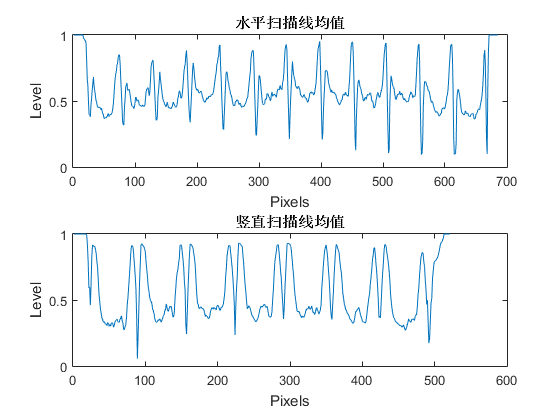
\includegraphics[width=0.7\textwidth]{bw_mean}
                    \caption{扫描线黑白均值}
                    \label{fig:bw_mean}
                \end{figure}

                周期性已经比较明显,块分界线(图\ref{fig:graycapture_bw}中的黑色直线)在扫描线黑白均值\ref{fig:bw_mean}中体现为\textbf{尖锐的低谷}。

                考虑用\texttt{findpeaks}函数获取这些低谷的位置,测试出性能较好的参数如下:

                \begin{table}[H]
                    \caption{\texttt{finkpeaks}函数参数设置}
                    \centering
                
                    \begin{tabular}{c|c|l}
                    \hline
                
                    \hline
                    \textbf{选项} & \textbf{值} & \textbf{作用} \\
                    \hline
                        \texttt{MinPeakProminence} & 0.3 & 筛选出较突出(尖锐)的峰值 \\
                    \hline
                        \texttt{MaxPeakWidth} & 10 & 去除过宽的峰值 \\
                    \hline
                        \texttt{MinPeakDistance} & 30 & 去除距离过近的峰值 \\
                    \hline
                
                    \hline
                    \end{tabular}
                \end{table}

                找到的峰值如下:

                \begin{figure}[H]
                    \centering
                    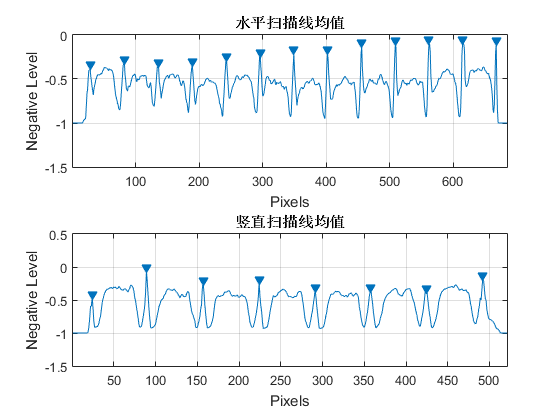
\includegraphics[width=0.7\textwidth]{findpeaks}
                    \caption{\texttt{findpeaks}检测峰值(纵坐标为原数据的相反数)}
                \end{figure}

                可见效果相当好,免去繁杂的傅里叶变换(若不能得当地处理噪声,傅里叶变换得到的结果不是特别准确)。

                \begin{minted}{matlab}
%% get block size and position of game region
hor = mean(image,1);
ver = mean(image,2);

[~,I] = findpeaks(-hor,'MinPeakProminence',0.3,'MaxPeakWidth',10,'MinPeakDistance',30);
[~,J] = findpeaks(-ver,'MinPeakProminence',0.3,'MaxPeakWidth',10,'MinPeakDistance',30);
Xs = I(1); Ys = J(1);
Wb = mean(diff(I)); Nc = length(I) - 1;
Hb = mean(diff(J)); Nr = length(J) - 1;
                \end{minted}

                得到结果\texttt{(Xs=28, Ys=24, Wb=53.33, Hb=66.86, Nc=12, Nr=7)},仍然运行代码\ref{code:all_blocks}绘制获取到的所有块。

                \begin{figure}[H]
                    \centering
                    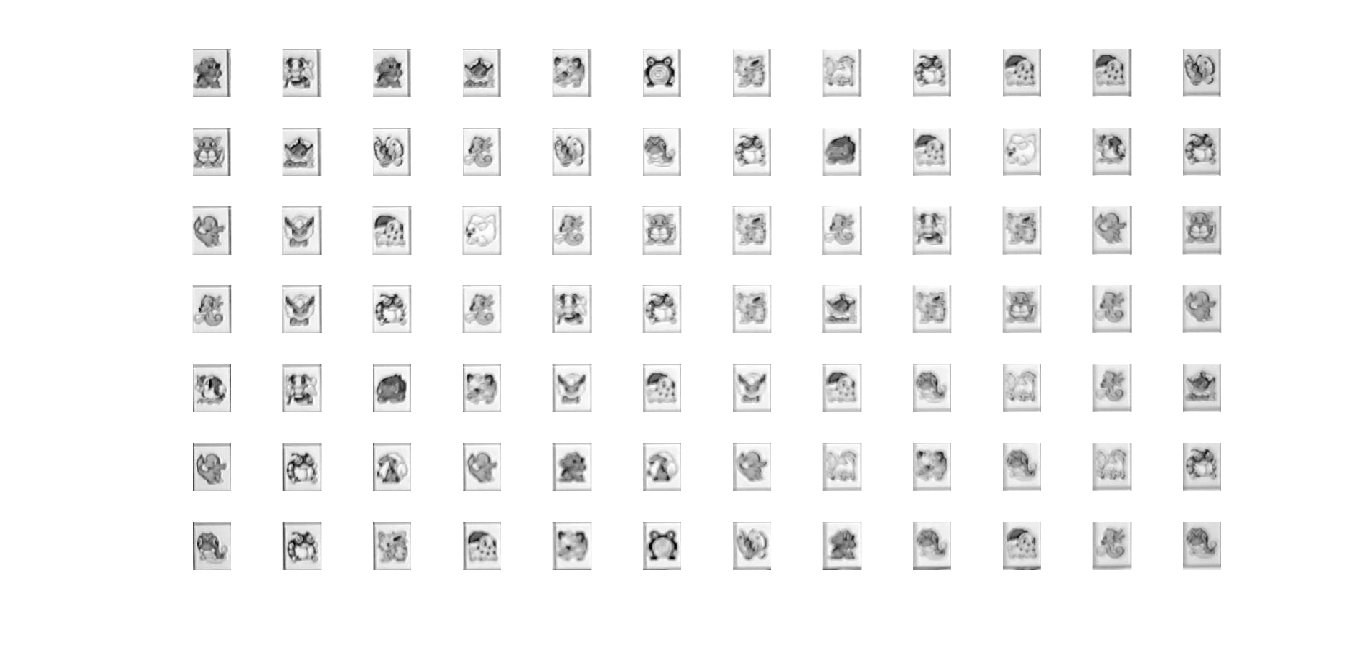
\includegraphics[width=\textwidth]{all_blocks_2}
                    \caption{利用二值图像法得到的图像分割效果}
                \end{figure}

                分割效果很好。若使用\textbf{二值图像法}重新对第一题的\texttt{graygroundtruth}进行处理,得到的尺寸参数为\texttt{(Xs=25, Ys=35, Wb=80, Hb=100, Nc=12, Nr=7)},与使用第一题方法得到的结果完全相同。\textbf{可见二值图像法对干净图像以及摄像头采集图像均有良好的性能。}

                \textbf{二值图像法}利用黑白图像的强对比度增强了图像的周期性,便于后续提取尺寸信息;若不转化为黑白图像,直接傅里叶变换可以看到基波频率附近有许多能量也很高的噪声频率分量,对识别基波频率的准确度有巨大影响。\textbf{二值图像法}虽然丢失了图像的细节,但增强了对分块影响最大的周期性,因此\textbf{二值图像法}用于分块不失为一种优越的方法。

            \item 在第2题基础上,计算所有图像分块的两两相似性,选出最相似的十对图像块。

                \begin{enumerate}
                    \item \textbf{高通滤波}:利用\texttt{imfilter}函数对图像进行高通滤波提取纹理特征。

                        \begin{minted}{matlab}
% ...

hp = [-0.3,-0.3,-0.3;
      -0.3, 0.5,-0.3;
      -0.3,-0.3,-0.3];     % construct high pass filter
  
N = length(blocks);
for i = 1:N
    im1 = imfilter(double(blocks{i})-128,hp);
    im1 = (im1-min(min(im1)))/(max(max(im1))-min(min(im1)))*255;

% ...
                        \end{minted}

                        \begin{figure}[H]
                            \centering
                            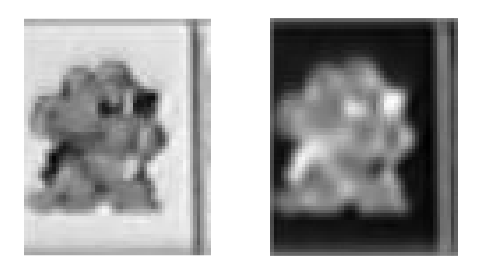
\includegraphics[width=\textwidth]{highpass}
                            \caption{高通滤波提取纹理特征}
                            \label{fig:highpass}
                        \end{figure}

                    \item \textbf{计算两图像相似度}:匹配滤波。

                        \begin{listing}[H]
                            \inputminted{matlab}{../process/similarity.m}
                            \caption{\texttt{similarity.m}}
                        \end{listing}

                    \item \textbf{两两计算相似度并排序}:二重循环暴力实现。

                        \inputminted{matlab}{../process/similarsort.m}
                        \begingroup
                            \captionof{listing}{\texttt{similarsort.m}}
                        \endgroup

                        \texttt{尽量使各图像块的灰度值均匀地分布在\texttt{0}的两侧(-128~127),这样在做相似度运算时,正负相消使得结果更准确了。}

                \end{enumerate}

                分别用\texttt{graygroundtruth}和\texttt{graycapture}测试,按相似度排序后,相似度走势曲线如图\ref{fig:similarity}。(两个\texttt{match\_map}分别存在\\
                \href{../process/graygroundtruth_match_map.mat}{\texttt{graygroundtruth\_match\_map.mat}}和\href{../process/graycapture_match_map.mat}{\texttt{graycapture\_match\_map.mat}}中)

                \begin{figure}[H]
                    \centering
                    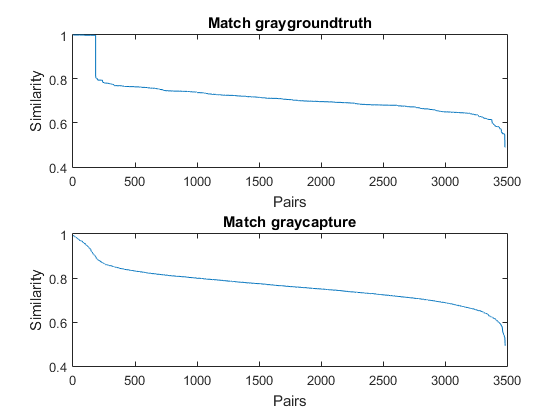
\includegraphics[width=0.7\textwidth]{similarity}
                    \caption{相似度走势曲线}
                    \label{fig:similarity}
                \end{figure}

                \begin{itemize}
                    \item 对于屏幕截图\texttt{graygroundtruth},相同两块的相似度几乎均为\texttt{1},而不同两块的相似度明显较低(低于\texttt{0.8});
                    \item 对于摄像头采集图像\texttt{graycapture},相似度曲线几乎是连续的,但在\texttt{Similarity=0.88}附近也出现了明显的拐点。
                \end{itemize}

                找出\texttt{graycapture}中相似度最高的十对图像块:

                \begin{minted}{matlab}
figure;

for i = 1:10
    subplot('position',[0.1+(i-1)*0.08,0.55,0.08,0.1]);
    imshow(blocks{match_map2(i,1)}); title(num2str(match_map2(i,3)));
    subplot('position',[0.1+(i-1)*0.08,0.35,0.08,0.1]);
    imshow(blocks{match_map2(i,2)});
end
                \end{minted}

                \begin{figure}[H]
                    \centering
                    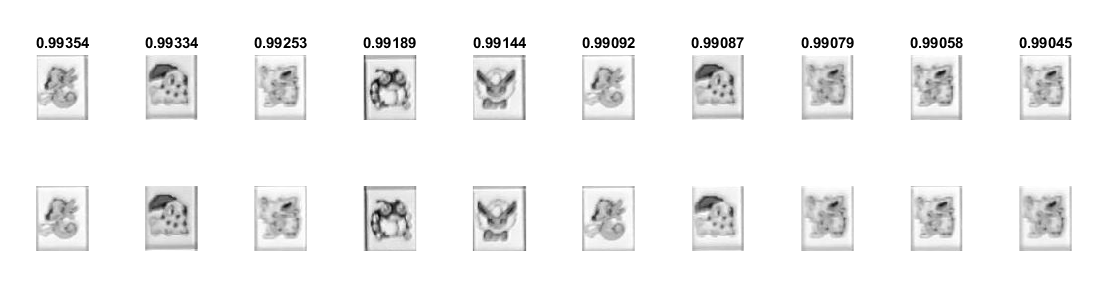
\includegraphics[width=\textwidth]{similarity10}
                    \caption{相似度最高的十对图像块}
                    \label{fig:similarity10}
                \end{figure}

                相似度最高的十对图像块确实是相同的图像块。

            \item 在第3题的基础上,找出相似度最大却不是同一种精灵的十对图像块。

                首先需手动标定各位置的精灵类别:

                \begin{table}[h]
                    \caption{精灵种类对应表(人脑识别)}
                    \label{tab:pokemon}
                    \centering
                
                    \begin{tabular}{c|c}
                    \hline
                
                    \hline
                    \textbf{序号} & \textbf{精灵} \\
                    \hline
                        1 & 小锯鳄 \\
                        2 & 大针蜂 \\
                        3 & 水精灵 \\
                        4 & 喵喵 \\
                        5 & 蚊香蛙 \\
                        6 & 尼多兰 \\
                        7 & 小火马 \\
                        8 & 芭瓢虫 \\
                        9 & 菊草叶 \\
                        10 & 巴大蝴 \\
                        11 & 杰尼龟 \\
                        12 & 墨海马 \\
                        13 & 绿毛虫 \\
                        14 & 妙蛙种子 \\
                        15 & 小海狮 \\
                        16 & 波波 \\
                        17 & 小火龙 \\
                        18 & 火精灵 \\
                        19 & 卡蒂狗 \\
                    \hline
                
                    \hline
                    \end{tabular}
                \end{table}

                \begin{listing}[H]
                    \begin{minted}{matlab}
kind = [1,  2,  1,  3,  4,  5,  6,  7,  8,  9,  9,  10;
        11, 3,  10, 12, 10, 13, 8,  14, 9,  15, 16, 8 ;
        17, 18, 9,  15, 12, 11, 6,  12, 2,  6,  17, 11;
        12, 18, 8,  12, 2,  8,  6,  3,  6,  11, 12, 17;
        16, 2,  14, 4,  18, 9,  18, 9,  13, 7,  12, 3 ;
        17, 8,  19, 17, 1,  19, 17, 7,  4,  13, 7,  8 ;
        13, 8,  6,  9,  4,  5,  10, 1,  13, 9,  12, 13;];
                    \end{minted}
                    \caption{手动标定精灵种类}
                    \label{code:classify_manually}
                \end{listing}

                找出十对不同但相似度最高的图像块:

                \begin{minted}{matlab}
figure;
count = 0;
kindt = kind.';

for i = 1:size(match_map2,1)
    if kindt(match_map2(i,1)) ~= kindt(match_map2(i,2))
        count = count + 1;
        subplot('position',[0.1+(count-1)*0.08,0.55,0.08,0.1]);
        imshow(blocks{match_map2(i,1)}); title(num2str(match_map2(i,3)));
        subplot('position',[0.1+(count-1)*0.08,0.35,0.08,0.1]);
        imshow(blocks{match_map2(i,2)});
        xlabel(['index:',num2str(i)]);
        if count == 10
            break
        end
    end
end
                \end{minted}

                \begin{figure}[H]
                    \centering
                    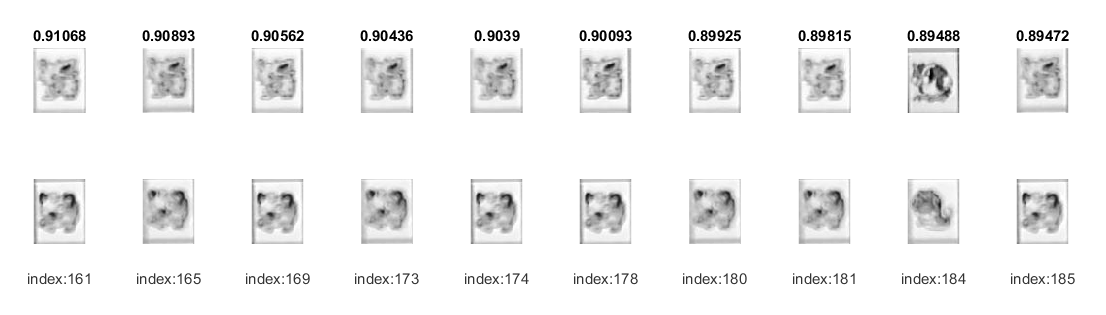
\includegraphics[width=\textwidth]{mistakes10}
                    \caption{不同块最相似前十名}
                    \label{fig:mistakes10}
                \end{figure}

                图\ref{fig:mistakes10}在每对图像块下方标注了它们在排序后\texttt{match\_map2}中的位置,这说明并非从某一位置开始起,后面的图像块均是不同块,至少在相似度\texttt{(0.89,0.91)}这一区间内,正确和错误的判断掺杂在了一起,这表明\textbf{摄像头采集图像的噪音使得算法可能发生误判}。而屏幕截图很少出现这样的问题。

                图\ref{fig:mistakes10}的结果和主观感受部分符合,惊人地发现前十名误判中有\texttt{90\%}是\textbf{尼多兰}和\textbf{喵喵},原因可能是轮廓较像且摄像头拍摄模糊(高通滤波使得细节丢失了)。

                \textbf{既然高通滤波丢失了一些细节信息,那么不做高通滤波,直接做相似度计算,结果如何呢?}对代码稍作修改,重复上述过程得到:

                \begin{figure}[H]
                    \centering
                    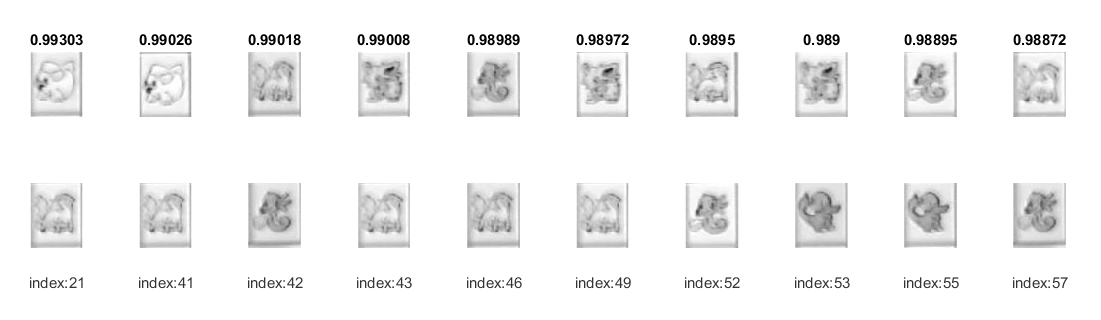
\includegraphics[width=\textwidth]{mistakes10-nohighpass}
                    \caption{不做高通滤波直接利用相似度匹配的误判前十名}
                    \label{fig:mistakes10_nohighpass}
                \end{figure}

                不做高通滤波使得重要的纹理特征被掩盖了,细节喧宾夺主,在相似度高达\texttt{0.99}时就发生了误判。这说明\textbf{高通滤波是至关重要的一步}。

                这也从另一方面说明了:\textbf{使用不同的高通滤波器也对判断结果有影响}。

            \item 在第3题基础上,将游戏区域映射为索引值的数组,并列出索引值和图像分块的对照关系表。

                在上一题中,已经手动做过这一步(表\ref{tab:pokemon}以及代码\ref{code:classify_manually}),现用程序实现,比较结果。

                分类函数\texttt{classify}:

                \inputminted{matlab}{../process/classify.m}
                \begingroup
                    \captionof{listing}{\texttt{classify.m}}
                \endgroup

                算法核心为以下几点:

                \begin{itemize}
                    \item 维护\texttt{isclassified}向量,长度为\texttt{N}(要分类元素总数),每个位置存储对应元素当前的类别,尚未分类用\texttt{0}表示;
                    \item 设定阈值\texttt{threshold},只对相似度高于阈值的\texttt{Pair}进行分类操作;
                    \item 具体分类时,若当前\texttt{Pair}的两个元素均未分类,则开辟新的类别;若两元素之一已分类,则将另一元素也加入该分类;若两元素已分至同一类别,则跳过;若两元素已分至不同类别,则将两类别合并;
                    \item 高于阈值的\texttt{Pair}全部处理完仍有元素未分类,则对未分类的元素遍历,寻找其相似度最高的分类添加。
                \end{itemize}

                根据图\ref{fig:similarity}可确定合适的阈值:

                \begin{minted}{matlab}
>> category1 = classify(match_map1,0.9,84);
>> category2 = classify(match_map2,0.92,84);
                \end{minted}

                分别对\texttt{graygroundtruth}和\texttt{graycapture}分类的结果均为\textbf{19个类别}。以\texttt{graycapture}为例可视化:

                \begin{minted}{matlab}
figure;

for i = 1:length(category2)
    subplot(5,5,i);
    C = category2{i};
    imshow(blocks{C(1)});
    title(['#',num2str(i),' Counts: ',num2str(length(C))]);
end
                \end{minted}

                \begin{figure}[H]
                    \centering
                    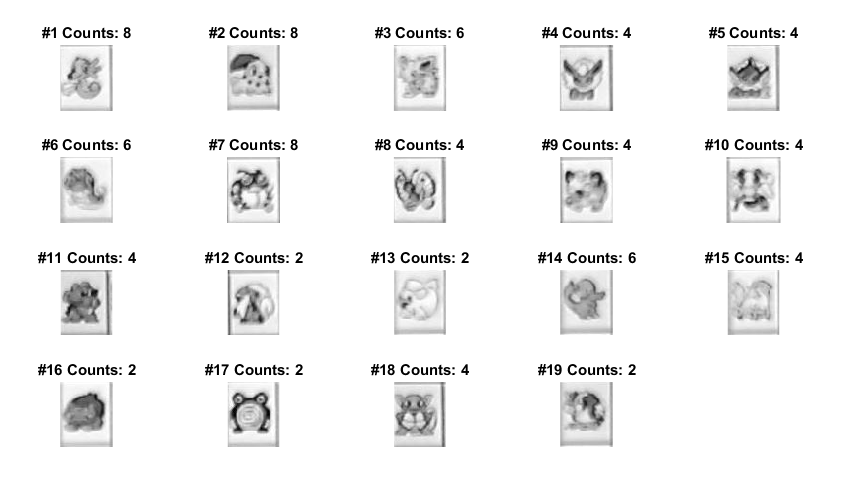
\includegraphics[width=0.8\textwidth]{category}
                    \caption{对\texttt{graycapture}自动分类结果}
                    \label{fig:category}
                \end{figure}

                与手动分类结果完全一致,正确率\texttt{100\%}。

                至此,可以得到游戏区域的\texttt{mtx}矩阵:

                \begin{minted}{matlab}
mtx = zeros(Nc,Nr);

for i = 1:length(category2)
    mtx(category2{i}) = i;  % rowwise index
end

mtx = mtx.';
                \end{minted}

            \item 在上述工作基础上,设计实现一个模拟的自动连连看。对摄像头采集的图像(灰度图像)\texttt{graycapture}进行分块并找出最相似的一对可消除分块后,将这图片上两个块的位置设为黑色或其他特定颜色(即模拟消除操作),并将图片展示在\texttt{figure}上。然后继续找出下一对可消除的分块并模拟消除,直至消除所有的分块或找不到可消除的分块对。

                首先对图像进行处理,获得游戏区域的\texttt{mtx}矩阵:

                \begin{listing}[H]
                    \inputminted[firstline=1,lastline=22]{matlab}{../process/mocklink.m}
                    \caption{\texttt{mocklink.m(1-22, get mtx)}}
                \end{listing}

                和之前的\href{../linkgame/canlink.m}{\texttt{canlink.m}}不同,这里进行模拟连接时不仅要考虑是否可以连接,我们还希望\textbf{函数能够返回相应的连接路径},进而绘制出连接路径,这样模拟连接的过程更真实。

                对\texttt{canlink}函数稍作修改得到\texttt{findpath}函数:

                \inputminted{matlab}{../process/findpath.m}
                \begingroup
                    \captionof{listing}{\texttt{findpath.m}}
                \endgroup

                相应地,将\texttt{omg.m}修改成为\href{../process/solvelinkgame.m}{\texttt{solvelinkgame.m}},增加了\texttt{connections}返回值,存储每次消除时连线的结点:

                \inputminted{matlab}{../process/solvelinkgame.m}
                \begingroup
                    \captionof{listing}{\texttt{solvelinkgame.m}}
                \endgroup

                最后是比较繁琐的可视化过程:

                \inputminted[firstline=22,lastline=74]{matlab}{../process/mocklink.m}
                \begingroup
                    \captionof{listing}{\texttt{mocklink.m(22-74, visualization)}}
                \endgroup

                连线为宽度为3像素的\textbf{黑线段},消去的块用白色背景表示。

                由于连线可能超出图像块的区域范围,需要特殊处理使得绘制出的连线仍在图片范围内。

                最终能够模拟消除能够正常工作,消除过程以动画形式保存为根目录下的\href{../mocklink.gif}{\texttt{mocklink.gif}}。

                以下取若干帧展示效果:

                \begin{figure}[H]
                    \centering
                    \begin{subfigure}{0.5\textwidth}
                        \centering
                        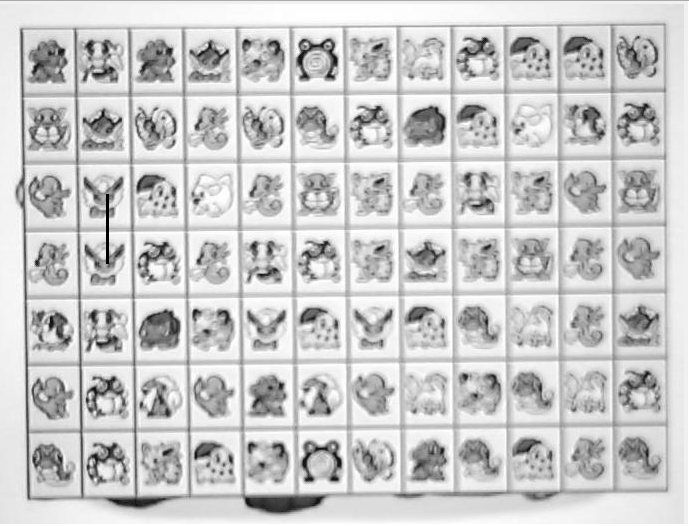
\includegraphics[width=0.8\linewidth]{mocklink1}
                    \end{subfigure}%
                    \begin{subfigure}{0.5\textwidth}
                        \centering
                        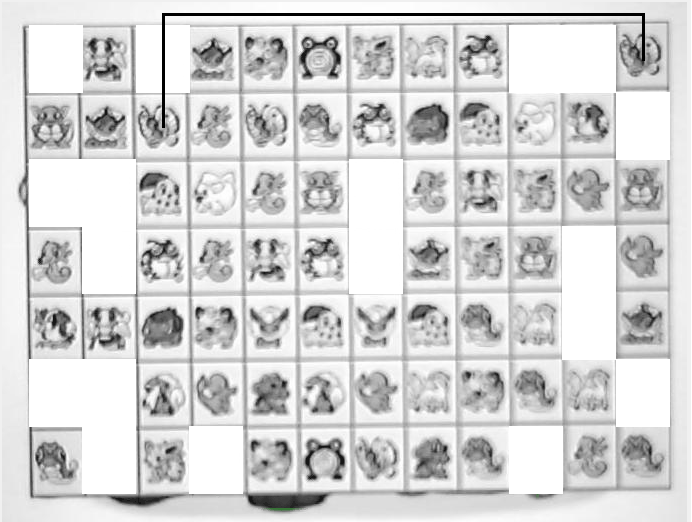
\includegraphics[width=0.8\linewidth]{mocklink2}
                    \end{subfigure}
                    \begin{subfigure}{0.5\textwidth}
                        \centering
                        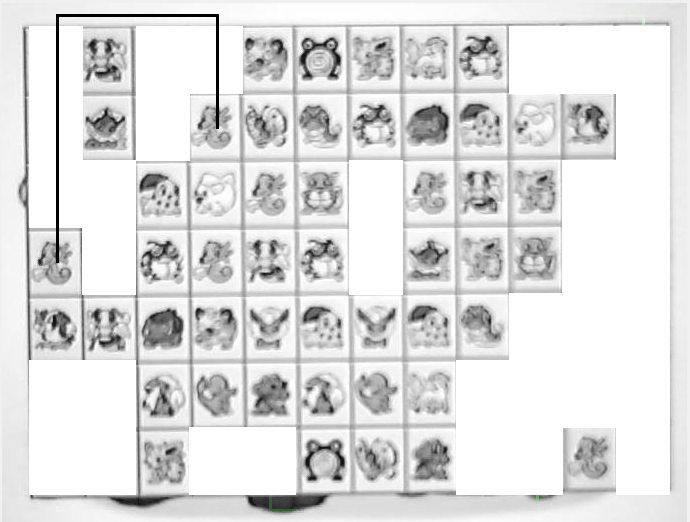
\includegraphics[width=0.8\linewidth]{mocklink3}
                    \end{subfigure}%
                    \begin{subfigure}{0.5\textwidth}
                        \centering
                        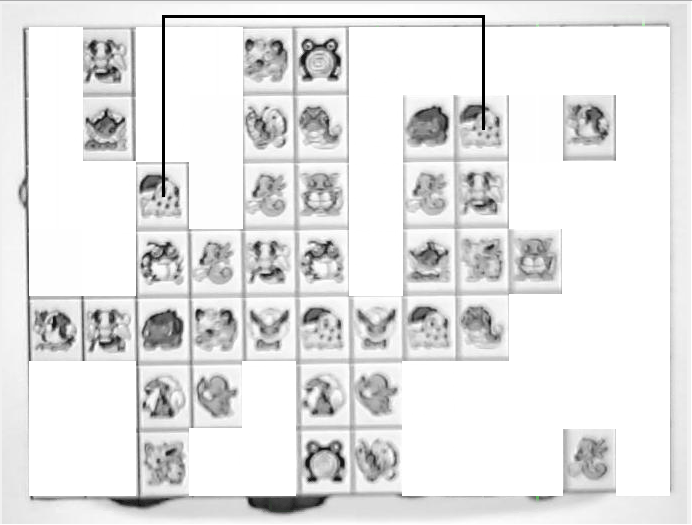
\includegraphics[width=0.8\linewidth]{mocklink4}
                    \end{subfigure}
                    \begin{subfigure}{0.5\textwidth}
                        \centering
                        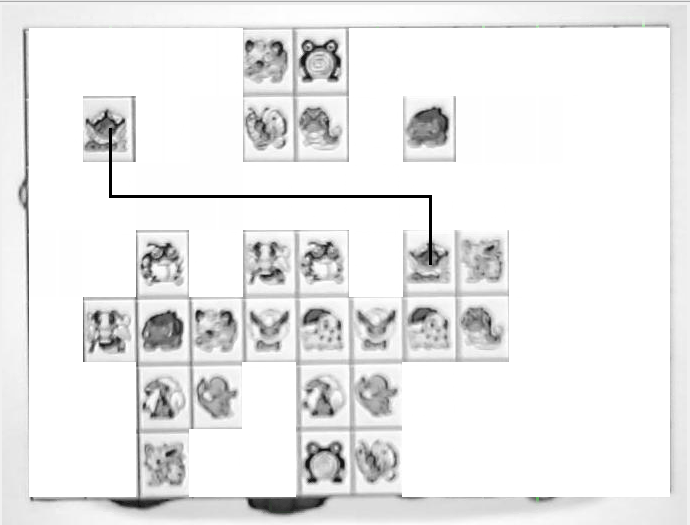
\includegraphics[width=0.8\linewidth]{mocklink5}
                    \end{subfigure}%
                    \begin{subfigure}{0.5\textwidth}
                        \centering
                        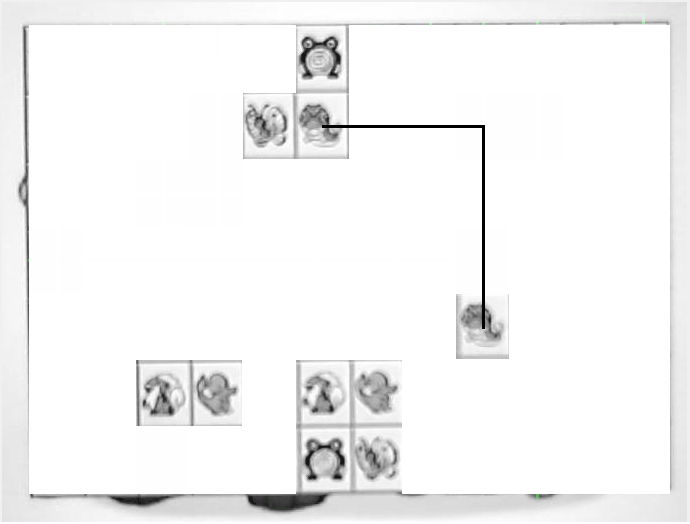
\includegraphics[width=0.8\linewidth]{mocklink6}
                    \end{subfigure}
                    \begin{subfigure}{0.5\textwidth}
                        \centering
                        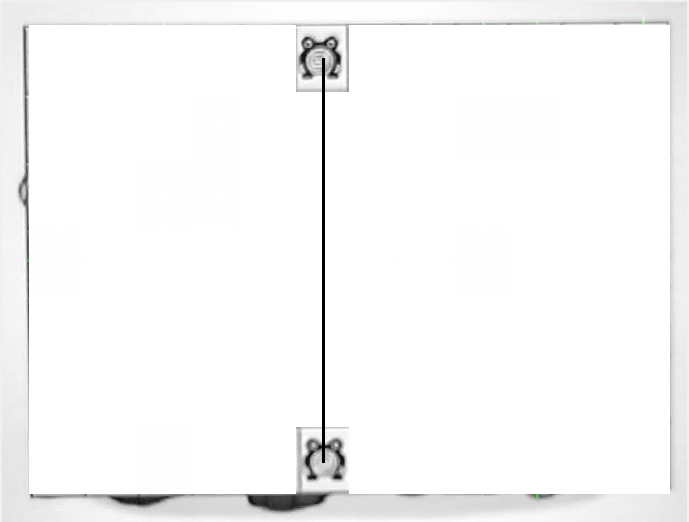
\includegraphics[width=0.8\linewidth]{mocklink7}
                    \end{subfigure}%
                    \begin{subfigure}{0.5\textwidth}
                        \centering
                        
\includegraphics[width=0.8\linewidth]{mocklink8}
                    \end{subfigure}
                    \caption{模拟消除过程(部分)}
                \end{figure}

        \end{enumerate}
    
    % section 攻克别人的连连看 (end)


\end{document}